%\documentclass[12pt, a4paper]{scrartcl}
%\usepackage[ngerman]{babel}
%\usepackage[utf8]{inputenc}

%\begin{document}
\section{Entwurf und Umsetzung der Netzwerk-Schnittstelle}
\subsection{Grundlegende Theorie zur Kommunikation in einem Netzwerk}
Unter dem Begriff Netzwerk im Zusammenhang mit dieser Arbeit wird, sofern nicht ausdrücklich anders definiert, die Ansammlung mehrerer, untereinander verbundener Computer verstanden.
Diese haben die Möglichkeit mit durch die ISO standardisierten Internet-Netzwerkprotokollen miteinander zu kommunizieren.\\ 

\begin{wrapfigure}{r}{.55\textwidth}
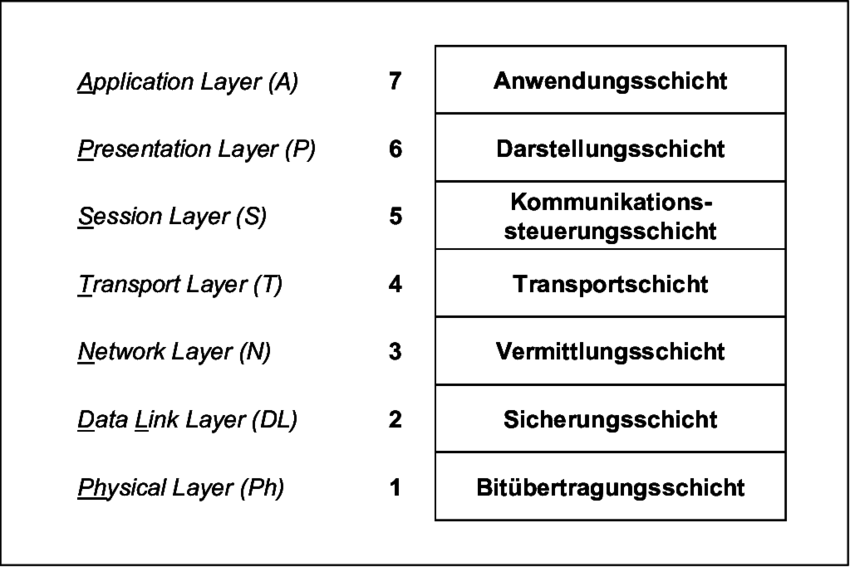
\includegraphics[scale=1]{isoosi}
\caption{Schematischer Aufbau des ISO/OSI-Modells\protect\footnotemark}
\label{ISOOSI}
\end{wrapfigure}
\footnotetext{https://www.researchgate.net/profile/Sebastian\_Lempert/publication/202268228/figure/fig1/\\AS:393996175200256@1470947416022/Abbildung-1-Die-7-Schichten-des-ISO-OSI-Referenzmodells-Der-geschichtete-Aufbau-eines.png [Zugriff: 20.12.2018 14:20 Uhr]}

Diese Kommunikation wird durch das ISO/OSI Modell beschrieben, auf dem auch die Arbeitsweise unseres Programmes aufbaut.
Innerhalb dieses Modells ist der Prozess einer Netzwerkübertragung sowie die dabei verwendeten Informationen bzw. Protokolle in Schichten nach ihrem Abstraktionsgrad einteilbar, von Nullen und Einsen in einem Kabel bis hin zu z.B. verschiedensten Verschlüsselungsprotokollen; was in unteren Schichten abgesichert ist, muss in denen darüber nicht implementiert werden, was wiederum zu einfachen und verlässlichen einzelnen Algorithmen in den Schichten führt, obwohl das gesamte System überaus komplex ist. 
Das Modell ist in Abbildung \ref{ISOOSI} dargestellt.

\subsection{Notwendigkeit, Anforderungen und Spezifikation eines eigenen Netzwerkprotokolls}
Um das Programm mit mehreren Programmierern zu entwickeln, muss eine gewisse Modularität gewährleistet werden. Außerdem müssen die Sinnabschnitte klar nach ihrer Funktion gegliedert sein und leicht benutzbare sowie wiederverwendbare Schnittstellen besitzen, damit nicht das gesamte Programm angepasst werden muss, wenn ein Teil geändert wird und jeder sich auf seinen Teil konzentrieren kann, ohne die anderen vollständig zu kennen.
Diese Anforderung wird durch die Trennung der verwendeten Programmiersprachen Lua und C++ einfach geregelt. Im C++ - Kontext muss es dennoch eine Unterteilung zwischen Netzwerkschnittstelle und Benutzeroberfläche geben, weshalb die gesamte Netzwerkkommunikation über eine statische Bibliothek in die ausführbare Datei eingebunden ist. 
Dort sind die Benutzeroberfläche und die Verbindung der Programmteile implementiert. 
Beide Programmteile nutzen die Funktionen und Klassen des frei zugänglichen Programmier-Frameworks Qt\footnote{https://www.qt.io/ [21.12.2018 16:30 Uhr]}.\\\\
Diese Netzwerkbibliothek stellt Funktionen und Klassen bereit, die eine verlässliche Verbindung zwischen zwei Rechnern aufbauen (Start und Ziel), über die ein erweiterbarer Satz von Anweisungen mit optionalen Argumenten sowie Dateien bidirektional übertragen werden können.
Startrechner bezeichnet daher immer den Rechner, vor dem der Anwender sitzt, Zielrechner denjenigen, der über das Programm gesteuert wird und Anweisungen erhält.\\
Dafür stellen sich folgende Anforderungen. Es muss:\\

\begin{itemize}
\item ein gesicherter Transport von beliebigen Daten möglich sein,
\item eine verschlüsselte Kommunikation vorliegen,
\item der Datenverkehr so klein wie möglich sein,
\item der Kommunikationskanal in beide Richtungen gleich aufgebaut sein,
\item die Übertragung von Dateien und Anweisungen möglich sein,
\item ein erweiterbares System zur Definition von Anweisungen existieren und
\item die Übertragung auch von größeren Dateien mit zusätzlichen Informationen fehlerfrei ablaufen.
\end{itemize}

Diese Bedingungen implizieren bereits, dass es eine bestimmte Regelung des Ablaufs für die Kommunikation zwischen den beiden Computern geben muss: ein Protokoll, also eine Kommunikationsvorschrift zwischen zwei Computern, das mit bestimmten Datenformaten und Abläufen das Verhalten der Computer während der Kommunikation festlegt.\par
Um nicht ebenfalls für die Ankunft der Daten selbst sorgen zu müssen, baut das Protokoll auf TCP/IP auf, genauer auf dem Protokoll TLS, welches schon eine verschlüsselte Verbindung bereitstellt, also der Sicherungsschicht des ISO/OSI-Modells. 
Demnach ist unser Protokoll zwischen der fünften und sechsten Schicht des Modells(s. Abb. \ref{ISOOSI}) einzuordnen, da es auf TLS aufbaut, aber noch nicht zur Darstellung von Informationen genutzt wird, wie es beispielsweise mit HTML der Fall wäre, sondern deren formatierte Übertragung und Aufbereitung zur Steuerung des Programms regelt.
Man kann die verschickten Daten in Pakete einteilen; das sind kleinere Datenabschnitte, die sequentiell, aber unabhängig voneinander verschickt und am Zielort zusammengesetzt werden.
Um diese Pakete innerhalb des Netzwerks zu navigieren, wird am Startcomputer an den Anfang jedes Pakets (\textit{Header}) ein Datensatz geschrieben, der Informationen zum Zielort, dem Weg oder der Behandlung der Daten des Pakets enthält.\\\par
Auf dieser Technik baut unser Protokoll auf. Es schreibt an den Anfang jeder Übertragung einen Datensatz mit einem festen Format, welcher die Art des Pakets beschreibt und am Zielort ausgelesen wird. Das bestimmt dann die weitere Behandlung der Daten.
Besonders im Fall von Anwendungen ist der Unterschied zwischen Header und Datenteil des Pakets fließend, da hier eine feste Struktur sowohl im Bezug auf die Größe als auch die Verarbeitungsgeschwindigkeit von Vorteil ist und die meisten Informationen zur Anweisung schon im Header integriert sind.
Da das Protokoll sowohl für den Versand von Anweisungen als auch von Dateien geeignet sein muss und dabei so strukturiert und einfach wie möglich soll, gibt es zwei verschiedene Teilprotokolle, was in dem folgenden Aufbau der Kommunikationsstruktur resultiert:\par
Im ersten Schritt werden zwei Informationen - nämlich der Typ der Übertragung, also Anweisung oder Datei, und ihre Gesamtgröße - in den Header des ersten Pakets der Übertragung geschrieben.\\
Abhängig davon, was der Übertragungstyp ist, werden nun entweder die Informationen für eine Datei- oder eine Anweisungsübertragung angehängt; die Gesamtgröße ermöglicht es die Vollständigkeit einer Übertragung zu verifizieren.
Dabei sind alle Werte, sofern es möglich ist, als Zahlen und nicht als Zeichenketten vorhanden, um die Größe der Informationen zu minimieren, und außerdem, besonders im Falle der Anweisungen, eine systematische Erweiterbarkeit zu gewährleisten.\\\par
Betrachtet man den Header für die Anweisungen, so ist zunächst ein Anweisungscode vonnöten, also eine vorher festgelegte Zahl für jede Anweisung.
Diese kann am Zielort eindeutig einer Handlungsfolge, d.h. einer bestimmten Anweisung zugeordnet werden.\\
Teil zwei sind Standardargumente, die binär auf 32 Bit Speicherbreite gesetzt werden können.
Diese Standardargumente sind dazu da, ein Zusammenfassen mehrerer ähnlicher Anweisungen zu gewährleisten und dadurch das Protokoll sinnvoll zu strukturieren, anstatt es mit Anweisungen zu überladen; so gibt es beispielsweise nur eine Anweisung um Ordnerstrukturen anzufordern.  
Mit ihr ist es möglich, die Dateien, die bereits auf dem Zielcomputer vorhanden sind, abzurufen und anzuzeigen. 
Je nachdem, welche Informationen zu welchen Dateien geschickt werden sollen, können jetzt Standardargumente als Bitflags gesetzt werden -  das bedeutet, die binäre Zahlendarstellung von Integern (Ganzzahlen) wird insofern ausgenutzt, dass einzelne Bits einer Ganzzahl mit bestimmter Speicherbreite auf eins oder null gesetzt werden können. Das kann am Zielort wieder ausgelesen werden und so dienen die Bits als "`Signale"', die die genaue Auslegung einer Anweisung bestimmen und dabei extrem platzsparend sind.
So können neben den Datei\-namen auch Dateigrößen, Zugriffsrechte oder andere Metainformationen mitgeschickt werden, wenn die entsprechenden Bits auf eins gesetzt worden sind - andernfalls wären dafür zusätzliche Anweisungen nötig, was das Protokoll unnötig vergrößern würde.\par
Der dritte Wert im Headersegment für die Anweisungen ist eine Zahl, die ein Programm identifiziert, auf das die Anweisung angewandt werden soll, was im Standardfall unsere Software ist.

\begin{figure}[h]
\begin{lstlisting}
     0                   1                   2                   3
     0 1 2 3 4 5 6 7 8 9 0 1 2 3 4 5 6 7 8 9 0 1 2 3 4 5 6 7 8 9 0 1
    +-+-+-+-+-+-+-+-+-+-+-+-+-+-+-+-+-+-+-+-+-+-+-+-+-+-+-+-+-+-+-+-+
    |                        Anweisungscode                         |
    +-+-+-+-+-+-+-+-+-+-+-+-+-+-+-+-+-+-+-+-+-+-+-+-+-+-+-+-+-+-+-+-+
    |                       Standardargumente                       |
    +-+-+-+-+-+-+-+-+-+-+-+-+-+-+-+-+-+-+-+-+-+-+-+-+-+-+-+-+-+-+-+-+
    |                        Zielprogramm-ID                        |
    +-+-+-+-+-+-+-+-+-+-+-+-+-+-+-+-+-+-+-+-+-+-+-+-+-+-+-+-+-+-+-+-+
    |             Länge des optionalen Arguments in Byte            |
    +-+-+-+-+-+-+-+-+-+-+-+-+-+-+-+-+-+-+-+-+-+-+-+-+-+-+-+-+-+-+-+-+
    |              optionales Argument variabler Länge              |
    +-+-+-+-+-+-+-+-+-+-+-+-+-+-+-+-+-+-+-+-+-+-+-+-+-+-+-+-+-+-+-+-+
\end{lstlisting}
\caption{Header für Anweisungen}
\label{Anweisungs_Header}
\end{figure}

Der vierte Wert ist eine Längenangabe in Byte.
Er bezeichnet die Länge des optionalen Paketinhalts beliebigen Formats, welches an den Header angehängt werden kann, beispielsweise ein Dateiname, ein Prüfungssummenwert oder ein Kommandozeilenbefehl.\par
Um die ganze Anweisung klein zu halten wird intern festgelegt, dass die Gesamtgröße dieses Headersegments inklusive des optionalen Arguments nicht größer als $2^{16}-1$ Byte sein darf - größere Anhänge müssen als Datei verschickt werden.
Aus Kompatibilitätsgründen mit verschiedenen Compilern und Systemen sind alle Zahlenwerte Integer(Ganzzahlen) mit 32 bzw. 64 Bit Speicherbreite angegeben, um damit sowohl genügend Platz für alle Informationen zu bieten als auch Probleme mit verschiedenen Anpassungen der Speicherbreite abhängig von der unterliegenden Rechnerarchitektur zu vermeiden, die während der Entwicklung ein Problem darstellten können.
Für den Nutzer spielen die tatsächlichen Kodierungen, also welches Programm oder welche Anweisung welchen Code erhält, keine Rolle. Sie werden intern festgelegt und bei  Interaktionen mit dem Nutzer ausgeführt oder in ihre Entsprechungen in von Menschen lesbare Form umgewandelt.
Die genauen Werte für Anweisung und Programme werden nur in seltenen Fällen im Zusammenhang mit der Nutzerseitigen Erweiterung des Anwendungskanons relevant, und sind im Anhang einsehbar.[s.S. \pageref{enums}]
Insgesamt ergibt sich die in Abbildung \ref{Anweisungs_Header} zu sehende Spezifikation des Headers für die Versendung von Anweisungen.
Dabei ist die Länge der Argumente in (pro Zeile 32) Bit angegeben, sofern nicht anders spezifiziert.\\\\
Das Versenden von Dateien hat andere Anforderungen, was in einem geänderten Aufbau des Header-Segments für die Übertragung, sowie in einem anderen Ablauf resultiert.\par
Für jede Dateiübertragung wird, im Gegensatz zu den Anweisungen, jeweils eine neue TLS-Verbindung aufgebaut, die unabhängig von den vorhergehenden und nachfolgenden ist. Es gibt also für jede Datei einen abgeschotteten "`Kanal"', in dem Fehler leicht behandelbar und konkurrierende Übertragungen unmöglich sind. 
Außerdem bleibt die Kennzeichnung einzelner Datenpakete erspart, was wiederum zu insgesamt weniger Datenverkehr führt.
Darauf folgend wird ein Paket mit Informationen zu der Datei zum Zielcomputer geschickt, welcher, um die Integrität der Übertragung zu verifizieren, dasselbe Paket zurücksendet.\\
Dieses Informationspaket ist in Abbildung \ref{Datei_Header} schematisch dargestellt.
Es besteht aus der Art der Datei (z.B. Video, Audio, Text, ausführbare Dateien etc.), was für die weitere Einordnung im Zielcomputer nützlich ist, dem ursprünglichen Datei\-namen und einer Prüfsumme, mit der die fehlerfreie Ankunft verifiziert werden kann. 
Auch hier spielt der tatsächliche Zahlenwert, der hinter dem Typ steht, nur intern eine Rolle, abgesehen von benutzerdefinierten Erweiterungen des Befehlssatzes, wie im Kapitel zur Eingabeverarbeitung nachzulesen ist. 
Deshalb sind die Codierungstabllen im Anhang enthalten. [s. S. \pageref{enums}]\\\\

\begin{figure}[h]
\begin{lstlisting}
	0                   1                   2                   3
    0 1 2 3 4 5 6 7 8 9 0 1 2 3 4 5 6 7 8 9 0 1 2 3 4 5 6 7 8 9 0 1
   +-+-+-+-+-+-+-+-+-+-+-+-+-+-+-+-+-+-+-+-+-+-+-+-+-+-+-+-+-+-+-+-+
   |                           Dateiart                            |
   |                                                               |
   +-+-+-+-+-+-+-+-+-+-+-+-+-+-+-+-+-+-+-+-+-+-+-+-+-+-+-+-+-+-+-+-+
   |                 Länge des Dateinamens in Byte                 |
   |                                                               |
   +-+-+-+-+-+-+-+-+-+-+-+-+-+-+-+-+-+-+-+-+-+-+-+-+-+-+-+-+-+-+-+-+
   |                  Länge der Prüfsumme in Byte                  |
   |                                                               |
   +-+-+-+-+-+-+-+-+-+-+-+-+-+-+-+-+-+-+-+-+-+-+-+-+-+-+-+-+-+-+-+-+
\end{lstlisting}
\caption{Header für Dateiübertragungen}
\label{Datei_Header}
\end{figure}

Das Headersegment ist so aufgebaut, dass zunächst die drei Ganzzahlwerte für Typ, Länge des Dateinamens in Byte und Länge der Prüfsumme in Byte in den Speicher geschrieben werden. 
Dann wird der Dateiname und die Prüfsumme angehängt und dieses gesamte Paket wird an den Zielcomputer übermittelt.\par
Ist die Verbindung verifiziert, wird mit der eigentlichen Übertragung der Datei begonnen, die in Abschnitten und ohne weitere Kennzeichnung in mehreren kleinen Paketen geschieht.
Das funktioniert, da unser Standard zum Einen auf TCP/IP aufbaut, welcher bereits die richtige Reihenfolge und Vollständigkeit der Pakete weitgehend sicherstellt und zum Anderen nur eine Verbindung pro Dateiübertragung aktiv ist.
Am Zielcomputer wird die Datei schließlich in einem temporären Standardverzeichnis abgespeichert und Paket für Paket zusammengesetzt.
Ist die Übertragung nach dem Senden einer bestimmten Bytesequenz vom Zielcomputer beendet, wird ein Signal aus einer der Managerklassen ausgesendet und die Verbindung getrennt.
Diese Schrittfolge ist schematisch in Abbildung \ref{file_diagram} dargestellt.
Die Aufgaben und Funktionen der Managerklassen werden im nächsten Kapitel genauer erläutert.
Nach der erfolgreichen Übertragung wird mit der anfänglich verschickten Prüfsumme der Datei ihre Integrität geprüft, um Fehler insgesamt auszuschließen, und die weitere Verarbeitung an die anderen Programmteile abgegeben.\\\\

\begin{wrapfigure}{r}{.6\textwidth}
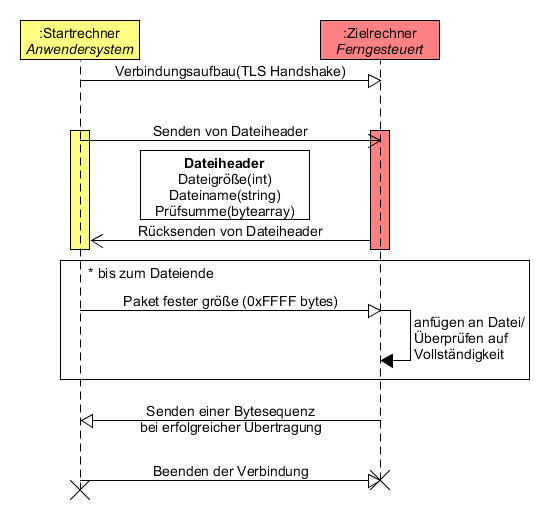
\includegraphics[scale=.5]{diagramFileProtocol}
\caption{Schematische Darstellung des Ablaufs bei der Dateiübertragung}
\label{file_diagram}
\end{wrapfigure}

Alle Anforderungen an das Protokoll werden erfüllt; der gesicherte und verschlüsselte Transport von Daten ist durch die Verwendung einer TLS-Verbindung und dem Aufbau eigener Kanäle erfüllt, die fehlerfreie Übertragung von Daten wird am Zielort über Gesamtgröße und Prüfsummen verifiziert, der Kommunikationskanal ist symmetrisch aufgebaut, da die Bibliothek sowohl für den Start- als auch für den Zielcomputer die nötige Funktionalität bereitstellt; die Codierung von allen Informationen als Zahlen oder als Bitflags sowie die Nutzung eigener Kanäle für Dateien reduziert den Datenverkehr drastisch, und damit ist auch dieser Punkt erfüllt, außerdem ist die Verwendung von Zahlencodes systematisch erweiterbar ohne die Speicherbreite verändern zu müssen, also wurden alle Ziele erreicht.

\subsection{Funktionsumfang der selbstgeschriebenen Netzwerkbibliothek}
Wie schon erwähnt, wird die Netzwerkkommunikation über eine statisch eingebundene Bibliothek vom Rest des Programmes abgetrennt.
Solch eine Bibliothek stellt die gesamte darin implementierte Funktionalität mit einigen wenigen, für den weitergehenden Gebrauch freigegebenen Funktionen und Klassen bereit.
Die Bibliothek stellt auf oberster Ebene eine Schnittstelle zum Übertragen von Dateien und Anweisungen zu einer bekannten Netzwerkadresse bereit.
Das heißt konkret, es werden Methoden der beiden Klassen MngThManager und MngFileManager bereitgestellt, welche die einzelnen Informationen intern in die zuvor spezifizierte Form umwandeln und verschicken sowie am Zielcomputer wieder entpacken und an die weiteren Programmteile übergeben.
Zusätzlich dazu ist eine entsprechende Fehlerbehandlung bei Verbindungsabbrüchen, fehlerhaften Übertragungen oder internen Kommunikationsproblemen durch falsche Eingaben sowie die Möglichkeit eine Fortschrittsmeldung bei der Dateiübertragung implementiert.
Insgesamt muss der Programmierer also nur mit zwei Klassen interagieren, um die volle Funktionalität der Bibliothek auszunutzen, weshalb sich das gesamte Konstrukt sehr gut für weitere Verwendungen in flexiblen Kontexten der modularen Programmierung eignet.

\subsection{Implementierung und Funktionsweise der Klassenbibliothek}

\begin{wrapfigure}{r}{.55\textwidth}
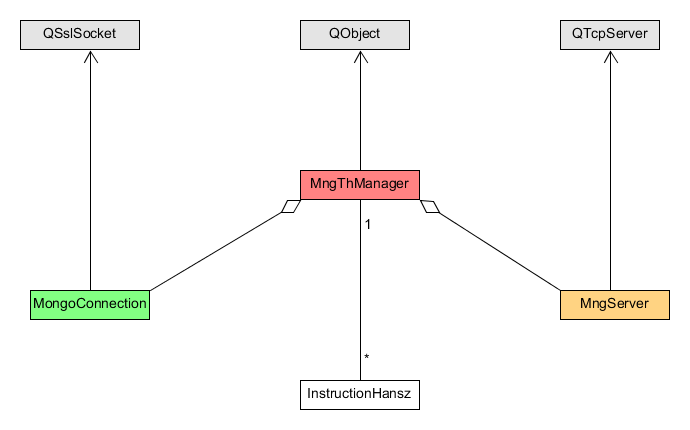
\includegraphics[scale=.4]{classDiagInstr}
\caption{Schematisch: Klassen zum Anweisungsversand}
\label{inst_d}
\end{wrapfigure}

In der Bibliothek sind neben den beiden oben genannten Manager-Klassen (MngThManager für Anweisungen und MngFileManager für Dateien) weitere Klassen definiert, die von den jeweiligen Manager-Klassen aus aufgerufen und benutzt werden und dadurch eine darunterliegende Schicht bilden, die durch eine fest definierte Schnittstelle an den Rest des Programms angebunden werden.
Außerdem gibt es eine von allen Klassen benutzte Datei, in der die Datenstrukturen und -typen, die in den Header der Pakete geschrieben werden, als C-Structs (s. \glsref{C-Structs}) definiert und einige Funktionen, die häufig gebraucht werden (z.B. String-Vervielfältigung, oder eine Funktion zum errechnen der Dateiprüfsumme) deklariert sind.\par
Der Aufbau der Übertragung beider Datentypen, die verschickt werden, ähnelt sich bis zu einem gewissen Punkt. 
So haben beide eine eigene Klasse, in der intern die Objekte (Anweisungen und Dateizugriffsobjekte) gespeichert sind und verwaltet werden (\textit{InstructionHansz} bzw. \textit{FileHansz}), sowie andere Klassen zum Verbindungsaufbau und dem Versand. 
So gibt es eine Klasse, die für das Annehmen von hereinkommenden Verbindungen zuständig ist und eine (bei Dateien zwei) Socket-Klassen (s. \glsref{Socket}), die sich um das Senden bzw. Empfangen von Daten kümmern, was in Abb. \ref{inst_d} bzw. \ref{file_d} vereinfacht schematisch dargestellt ist.\\

\begin{wrapfigure}{r}{.55\textwidth}
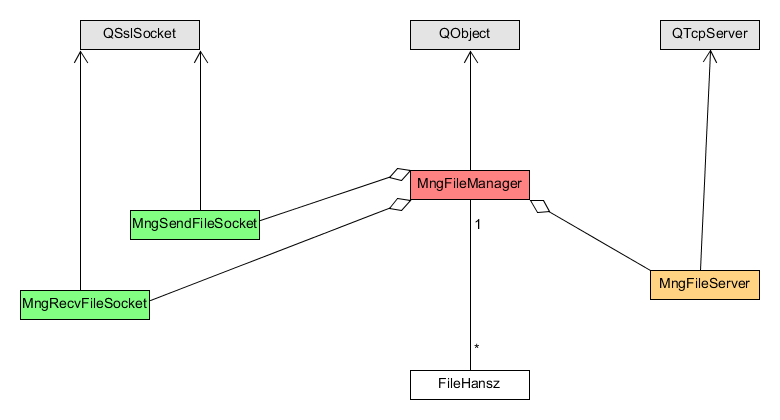
\includegraphics[scale=.35]{classDiagFile}
\caption{Schematisch: Klassen zum Dateiversand}
\label{file_d}
\end{wrapfigure}

Die beiden Speicherklassen werden dabei sowohl für den Empfang als auch das Senden eines Objektes genutzt - im ersten Fall werden sie mit den Teildaten (also Anweisungscode und zusätzlichen Argumenten oder Dateiname und Dateityp) initialisiert und erstellen daraus einen Pufferspeicher, der bereits den korrekten Header und das Datenpaket enthält, dessen Inhalt nur noch ausgelesen und verschickt werden muss - somit ist ein gleicher Aufbau der Verbindung in beide Richtungen sichergestellt.\par
Das tatsächliche Versenden sowie der Verbindungsaufbau wird von einer Server-Klasse und den Socket-Klassen übernommen.
Dabei horcht die Server-Klasse, sowohl für Dateien als auch für Anweisungen, auf der empfangenden Seite auf einem zuvor bestimmten Port auf eingehende Verbindungen.
Auf der sendenden Seite wird eine neue Klasse erstellt, welche ein TLS-Socket initialisiert und zu der gegebenen Adresse verbindet.
Ist die Verbindungsanfrage eingegangen, wird eine normale TLS-gesicherte Verbindung aufgebaut, sofern das möglich ist. 
Danach weichen die Abläufe von Dateiversand und Anweisungsübertragung ab: Anweisungen werden jetzt, in der Reihenfolge in der sie eingehen, von der Managerklasse an das Socket getaktet weitergeleitet, wo sie dann inklusive Header und Datenpaket verschickt werden - bei Dateien ist der Ablauf etwas komplexer.\\\par
Dabei muss zunächst erwähnt werden, dass für Dateien, im Gegensatz zu Anweisungen, jedes Mal eine neue Verbindung aufgebaut wird.
In der Verbindung für eine Datei wird, sobald sie aufgebaut ist, zuerst der Header für die Dateiübertragung an den Zielrechner gesendet, welcher genau dasselbe Paket dann zurückschickt um sicherzustellen, dass alle Steuerinformationen korrekt angekommen sind.
Jetzt startet die eigentliche Übertragung der Datei, welche mit dem Auslesen eines Datenblockes fester Größe beginnt.
Dieser wird in einen Pufferspeicher geschrieben, der, sobald er voll ist, von der Socket-Klasse ausgelesen und übertragen wird. 
Diese Anweisungsfolge wird so lange wiederholt, bis das Ende der Datei erreicht ist.
Der letzte Datenblock enthält oft weniger als die Maximalgröße, was aber in der Praxis kein Problem ist - das letzte Datenpaket auf der Seite des verschickenden Rechners ist nur etwas kleiner als der Rest.
Auf der empfangenden Seite werden die ankommenden Datenpakete über ihre Repräsentation als Filehansz-Objekt in eine nach ihrer Prüfsumme benannten Datei in einem temporären Verzeichnis gespeichert. 
Das verhindert die konkurrierende Benennung von ungleichen Dateien und vereinfacht das Überprüfen auf korrekte Übertragung. 
Die ursprünglichen Namen werden zu Beginn der Übertragung per Signal an das Programm außerhalb der Bibliothek geschickt, welches diese speichert - somit geht auch der Überblick nicht verloren.
Wurden alle Pakete verschickt und sind angekommen, wofür die TCP-basierte Verbindung sorgt, wird vom empfangenden Rechner eine Bytesequenz versendet, welche die erfolgreiche Übertragung kennzeichnet.\\\par
Danach wird die Verbindung beendet und die beiden Sockets gelöscht.
Der gesamte Prozess ist in Abb. \ref{file_diagram} (S. \pageref{file_diagram}) als Sequenzdiagramm dargestellt.\\
Die Verbindung für Anweisungen wird erst am Programmende oder bei einem disconnect-Befehl getrennt; sie läuft auf Port 16962, die Dateiübertragung auf Port 16963.
Greift man über das Internet auf einen Computer in einem lokalen Netzwerk zu, so muss zuvor beim Standardgateway für beide Ports Port-Forwarding eingestellt werden.\\\\
Insgesamt arbeiten die für den Benutzer der Schnittstellen nicht sichtbaren Klassen an der reibungslosen Funktion eines komplexen Protokolls, das sich durch extrem speichereffiziente Datenstrukturen und einen mehrstufigen Aufbau auszeichnet.
Dabei sind sie in ihrer Implementierung auf eine möglichst geringe Fehlerquote und Stabilität ausgelegt, insbesondere durch die Verwendung von einem "`Kanal"' pro Datei oder eine Taktung bei der Übertragung von Anweisungen, was das Abstürzen des Programms, das durch zu viele gleichzeitig geschickte Anweisungen entstünde, verhindert.
So entsteht ein stabiles und verlässliches System, welches die weitere Funktion unseres Programmes stützt.
%\end{document}